%-*- coding: UTF-8 -*-
% filename.tex
\documentclass[UTF8]{ctexart}
\usepackage{amsmath,mathtools,lmodern,hyperref, tikz}
\title{用到的公式}
\author{haodayizhia}
\date{\today}

\bibliographystyle{plain}

\begin{document}
\renewcommand\theequation{%
\thesection.\arabic{equation}}

\maketitle
\tableofcontents
\section{二体问题}

\subsection{核心公式}
\begin{equation}
	\ddot{\vec{r}}=-\frac{\mu}{r^3}\vec{r}
\end{equation}

\subsection{推导用到的向量公式}

\begin{gather}
\vec{a}\times(\vec{b}\times\vec c) =\vec{b}(\vec{a}\cdot\vec{c})-\vec{c}(\vec{a}\cdot\vec{b})\\
\vec{a}\cdot(\vec{b}\times\vec{c})=(\vec{a}\times\vec{b})\cdot\vec{c}
\end{gather}

\subsection{能量$E$守恒}
\begin{gather}
	\dot{\vec{r}}\cdot\ddot{\vec{r}}+\dot{\vec{r}}\cdot\frac{\mu}{r^3}\vec{r}=0\notag\\
	\to E=\frac{v^2}{2}+(c-\frac{\mu}{r})=\text{const}
\end{gather}

\subsection{角动量$\vec{h}$守恒}
\begin{equation}
	\vec{h}=\vec{r}\times\dot{\vec{r}}
\end{equation}

\subsection{近地点方向$\vec{B}=\mu\vec{e}$}
\begin{equation}
	\dot{\vec{r}}\times\vec{h}=\frac{\mu}{r}\vec{r}+\vec{B}
\end{equation}

\subsection[运动轨迹]{运动轨迹\footnote{不包含指向质心的直线降落}}
\begin{equation}
	r=\frac{h^2/\mu}{1+B/\mu\cos \theta}=\frac{p}{1+e\cos\theta}\\
\end{equation}

\begin{equation}
	r=
	\begin{cases}
		a & e=0,\text{圆}\\
		\frac{a(1-e^2)}{1+e\cos\theta} & 0<e<1,\text{椭圆}\\
		\frac{p}{1+\cos\theta} & e=1,\text{抛物线}\\
		\frac{a(e^2-1)}{1\pm e\cos\theta} & 1<e,\text{双曲线}
	\end{cases}
\end{equation}

以椭圆为例

\begin{center}
\centering
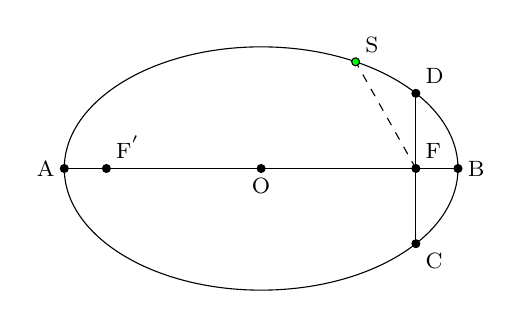
\begin{tikzpicture}
	\draw[black] (0, 0) ellipse(2.5 and 1.545);
	\draw[fill=black] (-2.5, 0) circle(0.05) node[left]{\footnotesize A};
	\draw[fill=black] (2.5, 0) circle(0.05) node[right]{\footnotesize B};
	\draw[fill=black] (0, 0) circle(0.05) node[below]{\footnotesize O};
	\draw[fill=black] (1.965, 0) circle(0.05) node[above right]{\footnotesize F};
	\draw[fill=black] (-1.965, 0) circle(0.05) node[above right]{\footnotesize F$^{'}$};
	\draw[fill=black] (1.965, -0.955) circle(0.05) node[below right]{\footnotesize C};
	\draw[fill=black] (1.965, 0.955) circle(0.05) node[above right]{\footnotesize D};
	\draw (-2.5, 0)--(2.5, 0);
	\draw (1.965, -0.955)--(1.965, 0.955);
	\draw[dashed] (1.965, 0)--(1.2, 1.355);
	\draw[fill=green] (1.2, 1.355) circle(0.05) node[above right]{\footnotesize S};
\end{tikzpicture}
\end{center}

\begin{center}
	F: prime focus, 代表中心天体\quad F$^{'}$: secondary/vacant focus\\
	AB: major axis, 长度为$2a$\quad F$^{'}$: focal distance, 焦距, 长度为$2c$\\
	CD: latus rectum, 长度为$2p$\\
	A: apoapsis(apogee/aphelion/aposelenium)\\
	B: periapsis(perigee/perihelion/periselenium)
\end{center}

\subsection{活力公式}
取近地点代入能量积分中
\begin{equation}
	\frac{1}{2}v^2-\frac{\mu}{r}=-\frac{\mu}{2a}
\end{equation}

\subsection{anomaly转换}

$\theta$: True anomaly(真近点角), $E$: Eccentric anomaly(偏近点角), $M$: Mean anomaly(平近点角).

\begin{gather}
	a-r=ae\cos E\\
	M=n(t-\tau)=E-e\sin E
\end{gather}

\subsection{Conversion between rv and classical orbit elements}
\paragraph{$rv$ to $\sigma$(注意$\arccos$)}
\begin{equation}
	\begin{cases}
		e=\frac{|\dot{\vec{r}}\times\vec{h}-\frac{\mu}{r}\vec{r}|}{\mu}\\
		a=\frac{h^2}{\mu(1-e^2)}\\
		i=\arccos{\frac{\vec{h}\cdot(0,0,1)}{h}}\\
		\Omega=\arccos\frac{(0,0,1)\times\vec{h}\cdot(1,0,0)}{|(0,0,1)\times\vec{h}|}\\
		\omega=\arccos\frac{\vec{B}\cdot((0,0,1)\times\vec{h})}{B|(0,0,1)\times\vec{h}|}\\
		\theta=\arccos\frac{\vec{r}\cdot\vec{B}}{rB}
	\end{cases}or
\begin{cases}
	a=-\frac{\mu r}{v^2r-2\mu}\\
	e=\sqrt{1-\frac{h^2}{\mu a}}\\
	i=\arccos{\frac{\vec{h}\cdot(0,0,1)}{h}}\\
	\Omega=\arccos\frac{(0,0,1)\times\vec{h}\cdot(1,0,0)}{|(0,0,1)\times\vec{h}|}\\
	\omega=\arccos\frac{\vec{B}\cdot((0,0,1)\times\vec{h})}{B|(0,0,1)\times\vec{h}|}\\
	\theta=\arccos\frac{\vec{r}\cdot\vec{B}}{rB}
\end{cases}
\end{equation}
\paragraph{$\sigma$ to $rv$}
\begin{equation}
	\begin{cases}
			A=\begin{bmatrix}
			\cos(-\Omega) & \sin(-\Omega) & \\
			-\sin(-\Omega) & \cos(-\Omega) & \\
			& & 1
		\end{bmatrix}\begin{bmatrix}
			1 & &\\
			& \cos(-i) & \sin(-i)\\
			& -\sin(-i) & \cos(-i)
		\end{bmatrix}\begin{bmatrix}
			\cos(\omega+\theta) & \sin(\omega+\theta) & \\
			-\sin(\omega+\theta) & \cos(\omega+\theta) &\\
			& & 1
		\end{bmatrix}\\
		\vec{r}=A\begin{bmatrix}
			\frac{p}{1+e\cos\theta}\\
			0\\
			0
		\end{bmatrix}\\
		\vec{v}=A\begin{bmatrix}
		\frac{he\sin\theta}{p}\\
		\frac{h(1+e\cos\theta)}{p}\\
		0
		\end{bmatrix}
	\end{cases}
\end{equation}
\bibliography{math}
\end{document}